\section{Warehouse}

The warehouse is responsible for moving product from receiving to shipping.

\subsection{Picking}

Orders are printed out on demand or in batches and assigned to pickers to be assmbled for the packers.

\subsubsection{Importing Orders}

\index{ERP-One Commands!ORDIMP}

Orders that have been placed through the online order management system must first be imported into ERP-ONE before they can be printed. Perform all the following steps from within the RDP session connected to \textbf{WT-RDS01}

\begin{enumerate}
	\item Login to website
	\item Download orders to import directory
	\item Run \texttt{ORDIMP}
\end{enumerate}

\paragraph{Logging into the website}

Before you can retrieve the orders from the website, you must log in.

\begin{figure}[H]
	\centering
	\begin{subfigure}[b]{0.4\textwidth}
		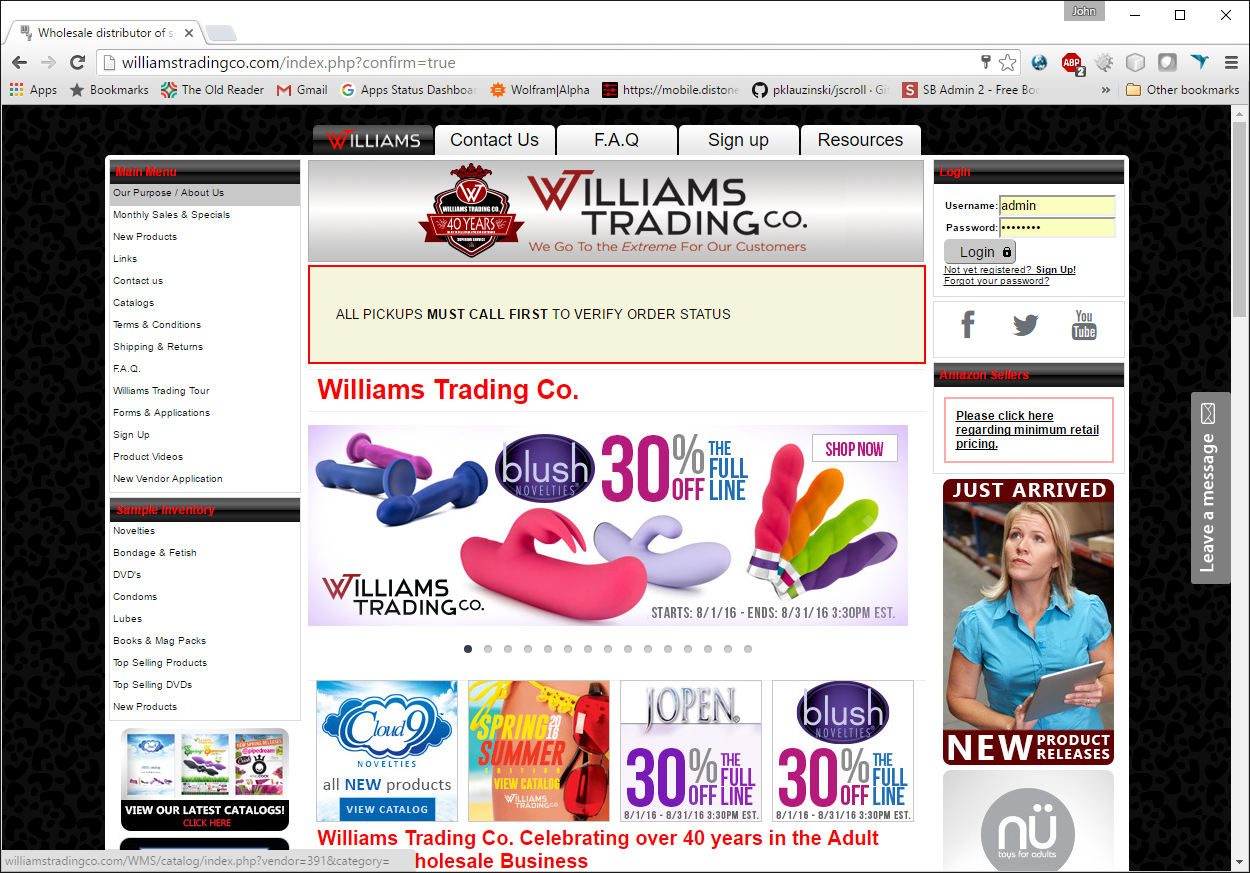
\includegraphics[width=\textwidth]{../img/image48}
		\caption{{\tiny WILLIAMSTRADINGCO.COM}}
	\end{subfigure}
	~
	\begin{subfigure}[b]{0.4\textwidth}
		
\includegraphics[width=\textwidth]{../img/image47}
		\caption{{\tiny MUFFSANDCUFFS.COM}}
	\end{subfigure}
	\caption{Logging into the website}
\end{figure}

\paragraph{Downloading orders to import directory}

After logging in, navigate to \textbf{Administrator} $\rightarrow$ \textbf{Manage Orders} $\rightarrow$ \textbf{Export Orders}


\begin{figure}[H]
	\centering
	\begin{subfigure}[b]{0.4\textwidth}
		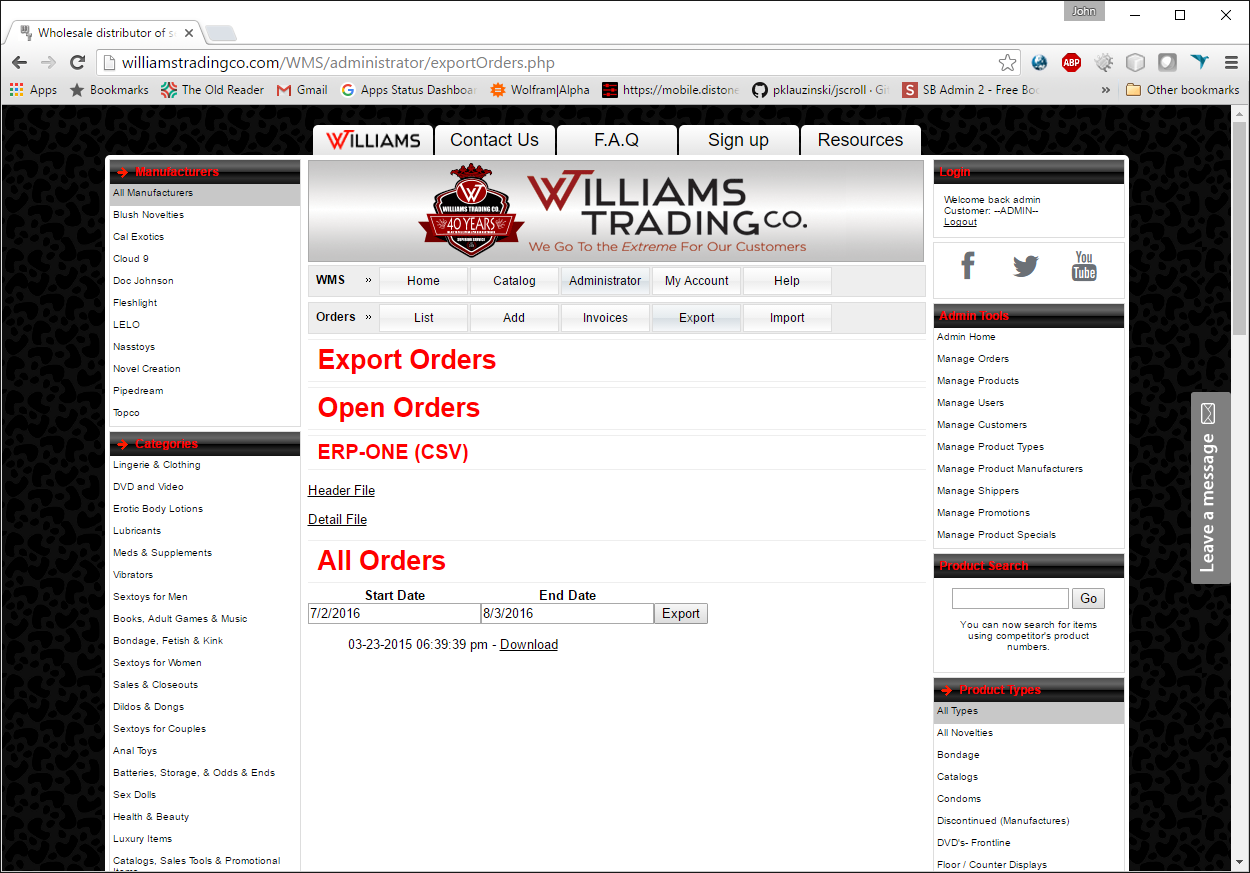
\includegraphics[width=\textwidth]{../img/image49}
		\caption{{\tiny WILLIAMSTRADINGCO.COM}}
	\end{subfigure}
	~
	\begin{subfigure}[b]{0.4\textwidth}
		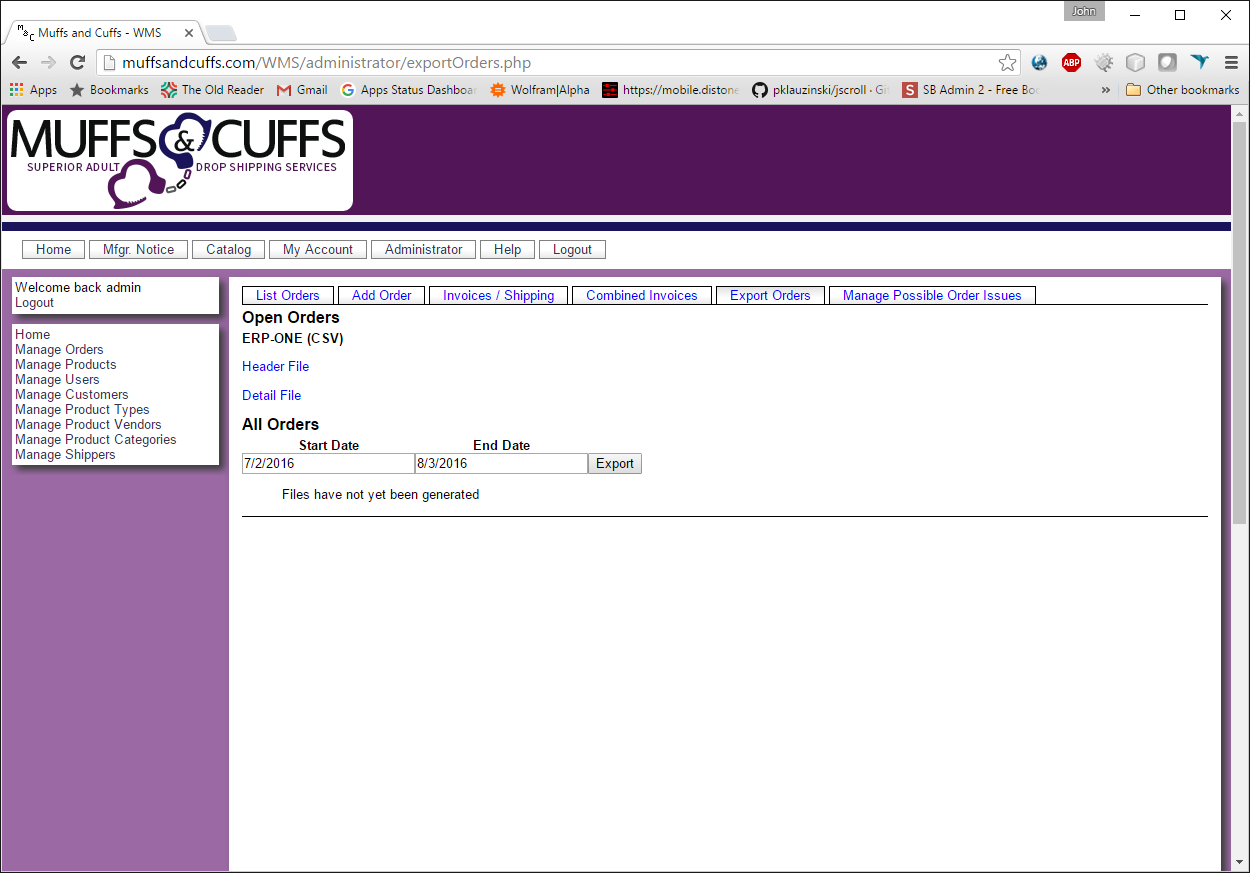
\includegraphics[width=\textwidth]{../img/image50}
		\caption{{\tiny MUFFSANDCUFFS.COM}}
	\end{subfigure}
	\caption{Exporting Orders}
\end{figure}

Right click on the file you wish to download and choose \textbf{"Save Link As..."} if you are in Chrome, or \textbf{"Save Target As..."} in Internet Explorer. A save dialog will open. 

Navigate to the E:{\textbackslash}WEB directory and save the files as \textbf{header.txt} and \textbf{detail.txt}.

If the files already exist, you should first confirm that no one is currently trying to import orders. After you have confirmed that no one else is trying to import orders, you may overwrite the files by clicking on either header.txt or detail.txt and clicking save. If you receive an error regarding permissions you must contact the administrator to have these files removed.

\paragraph{Peforming the import}

After the files have been placed in the correct directory, you may now perform the import by opening \texttt{ORDIMP} and clicking \textbf{Import\textsl{}}.

\begin{figure}[H]
	\centering
	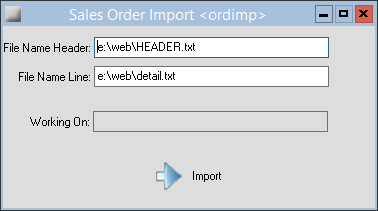
\includegraphics[width=0.5\textwidth]{../img/image46}
	\caption{ORDIMP Import}
\end{figure}\textsl{}

\subsubsection{Printing Pick Lists}

\index{ERP-One Commands!OEPS}

Pick lists are printed using the \texttt{OEPS} command in ERP-ONE

\begin{figure}[H]
	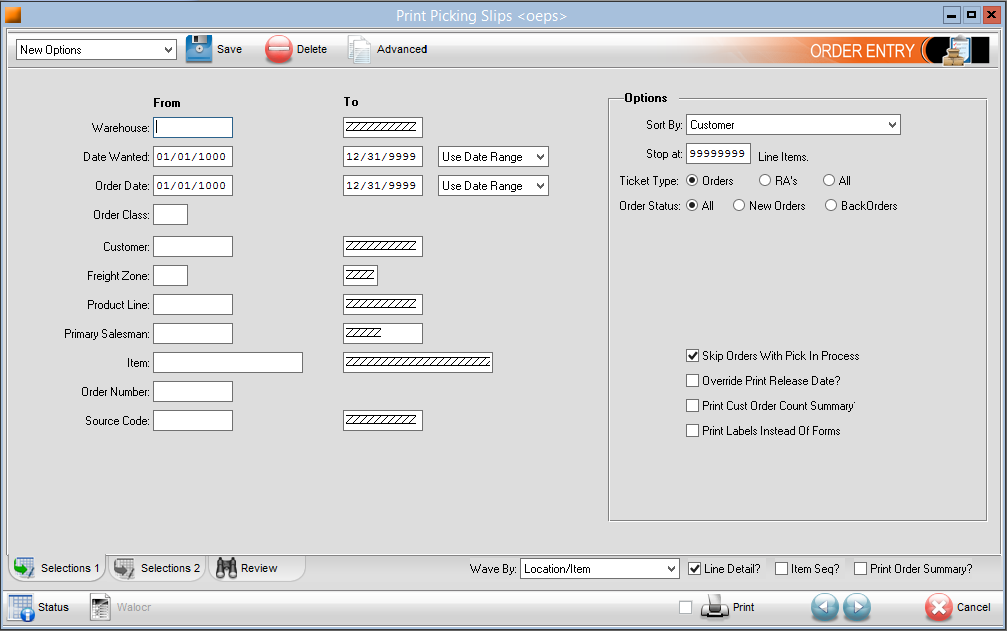
\includegraphics[width=\textwidth]{../img/image1}
	\caption{Selection screen of OEPS}
\end{figure}

Options on the first selection screen allow the warehouse manager to return a limited selection of orders ready to print. The \texttt{Wave By} option may be changed depending on how the orders are to be picked.

\begin{figure}[H]
	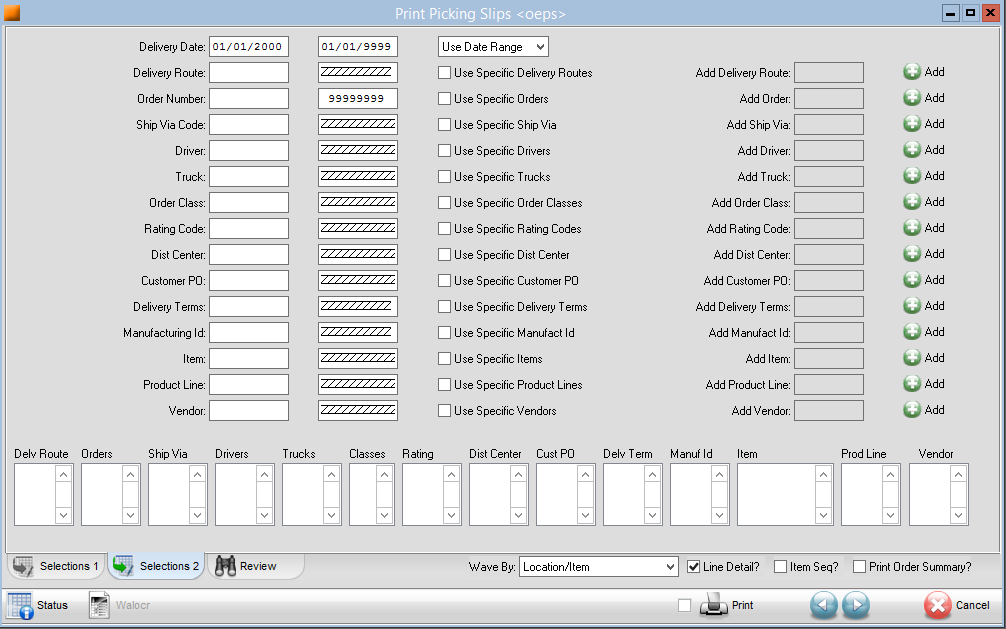
\includegraphics[width=\textwidth]{../img/image2}
	\caption{Additional selection screen of OEPS}
\end{figure}

Options on the second selection screen allow further filtering of orders that will appear on the review screen.

\begin{figure}[H]
	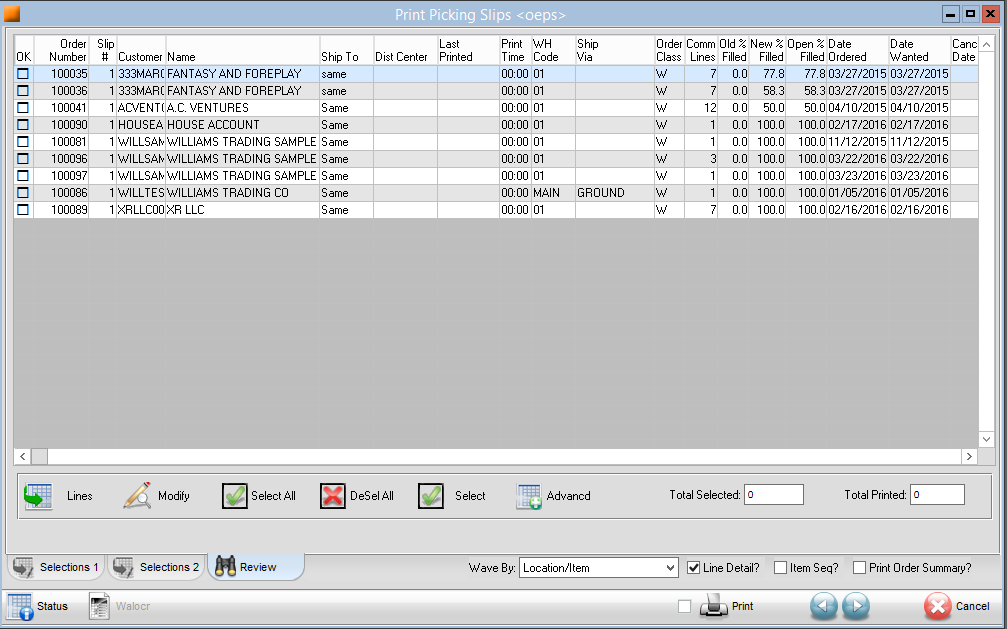
\includegraphics[width=\textwidth]{../img/image3}
	\caption{Review screen of OEPS}
\end{figure}

The review screen is where the warehouse manager will choose which orders they wish to print.  This can be done individually or using the \texttt{Select All} button. If further filtering is required clicking \texttt{Advanced} will pull up the following screen.

\textbf{NOTE} Printing a pick list reserves inventory for that order. Do not print pick lists that are not ready to be picked.

\begin{figure}[H]
	\centering
	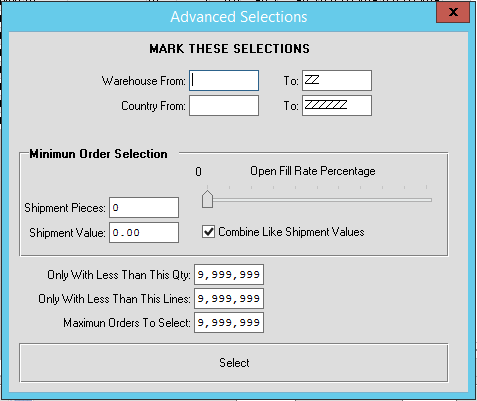
\includegraphics[width=0.5\textwidth]{../img/image4}
	\caption{Advanced selection screen of OEPS}
\end{figure}

\subsubsection{Picking Orders}

\begin{figure}[H]
	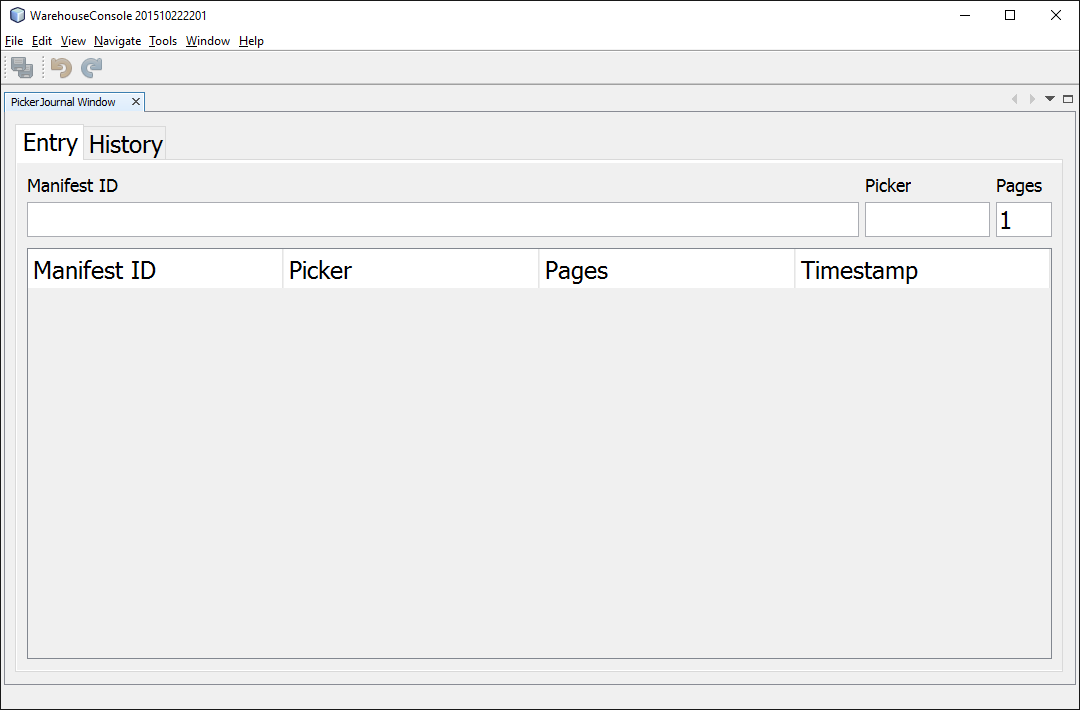
\includegraphics[width=\textwidth]{../img/image51}
	\caption{Warehouse Console Picking Log}
\end{figure}

Before they head into the aisles pickers must first scan their order(s) into the picker management terminal outside of the warehouse management office.  This ensures that accountability is maintained and the picker is known to be responsible for the order they have been assigned.

\pagebreak

\subsection{Packing}

Orders that have been picked from the aisles are delivered to the packing stations in shopping carts or totes containing multiple bins.  Carts may contain multiple orders, or be a part of a larger order.  Each bin in a tote will be a single order.

\index{ERP-One Commands!UCC}

Packers use the \texttt{UCCSS} command to verify items and print out the \emph{UCC} label which is later used for shipping.

\begin{figure}[H]
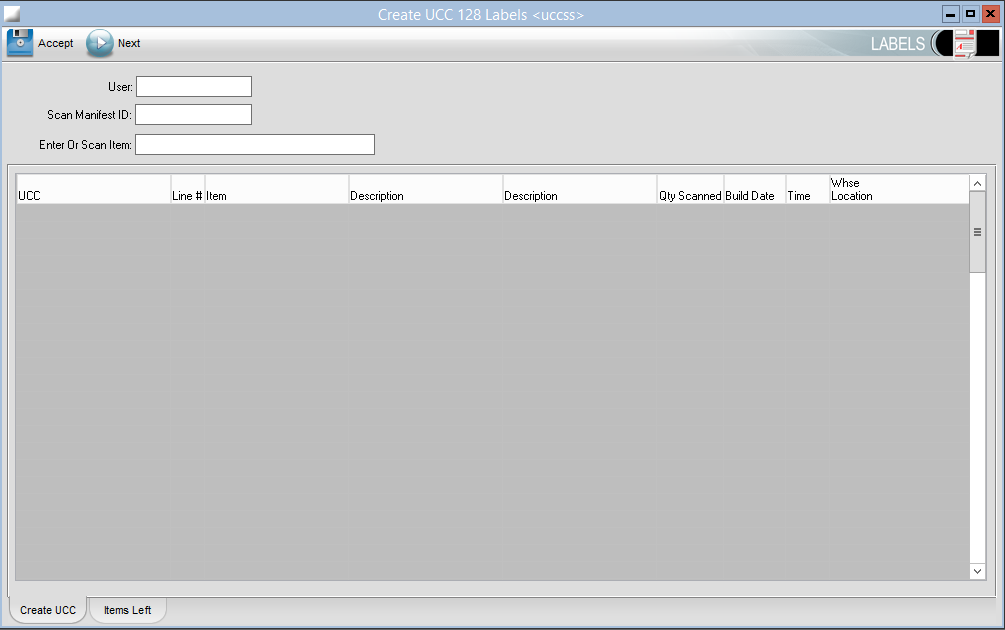
\includegraphics[width=\textwidth]{../img/image40}
\caption{UCC Scan Shipping}
\end{figure}

\begin{figure}[H]
	\centering
	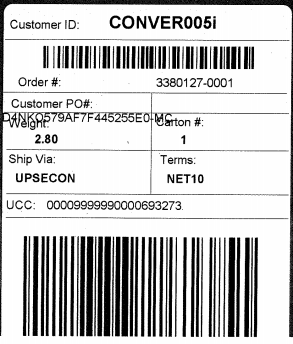
\includegraphics[width=0.5\textwidth]{../img/image42}
	\caption{UCC Box Label}
\end{figure}

The UCC box label is to be applied to the top of the carton so it can be read by the \textbf{CubiScan}.

\pagebreak

\subsection{Shipping}

Shippers are responsible for scanning the package identifier that has been affixed to the box by the packer.  They will utilize \textbf{ConnectShip}, or alternatively \textbf{Endicia Professional} or \textbf{Worldship} to print the shipping label.

\subsubsection{ConnectShip}

ConnectShip is a complete manifesting / shipping solution. Order and package information is available to ConnectShip from ERP-ONE and the CubiScan database. Packages that have traveled through the conveyor belt will have been weighed and dimensioned. Packages that have not traveled through the belt (i.e. envelopes) will need to be weighed at the shipping terminal.

\begin{figure}[H]
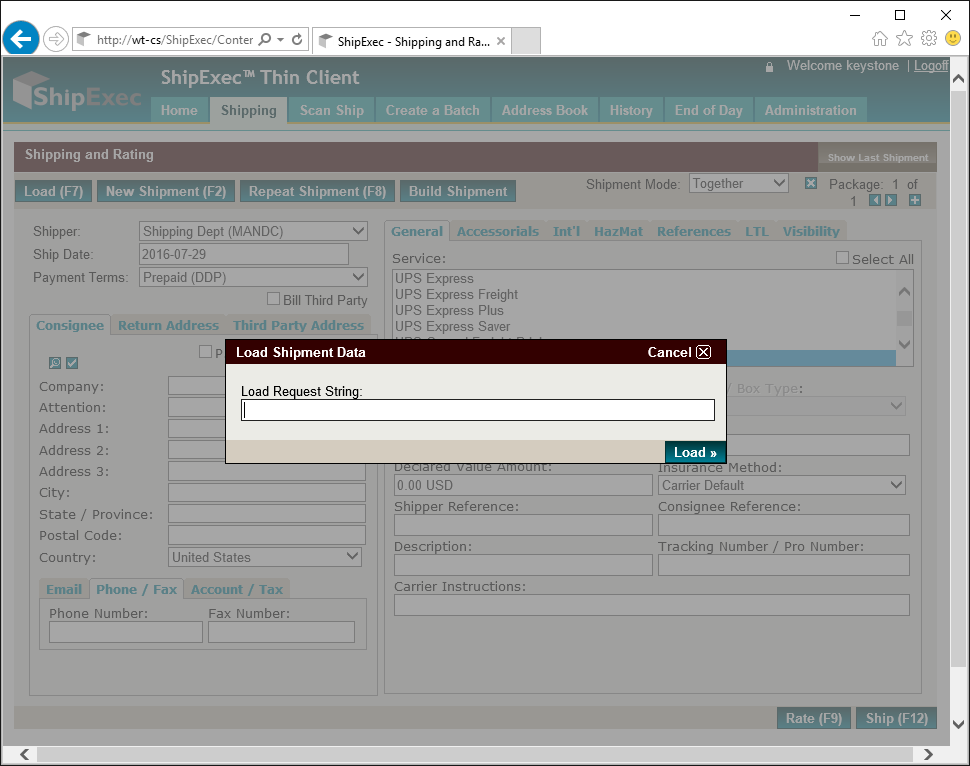
\includegraphics[width=\textwidth]{../img/image43}
\caption{ConnectShip Load Shipment Data}
\end{figure}

ConnectShip is responsible for chosing and printing the appropriate shipping service for each package.  The user is expected to be able to scan the Order ID from the UCC label that was affixed by the packer, and ConnectShip will retreive all necessary information. The user then does a visual confirmation of the options selected and is then able to press \texttt{F12} or use the mouse to click \texttt{Ship}.  The shipping label will print out and they will apply it to the package. In the case of envelopes the envelope must be placed on the scale before the ship button is pressed

\begin{figure}[H]
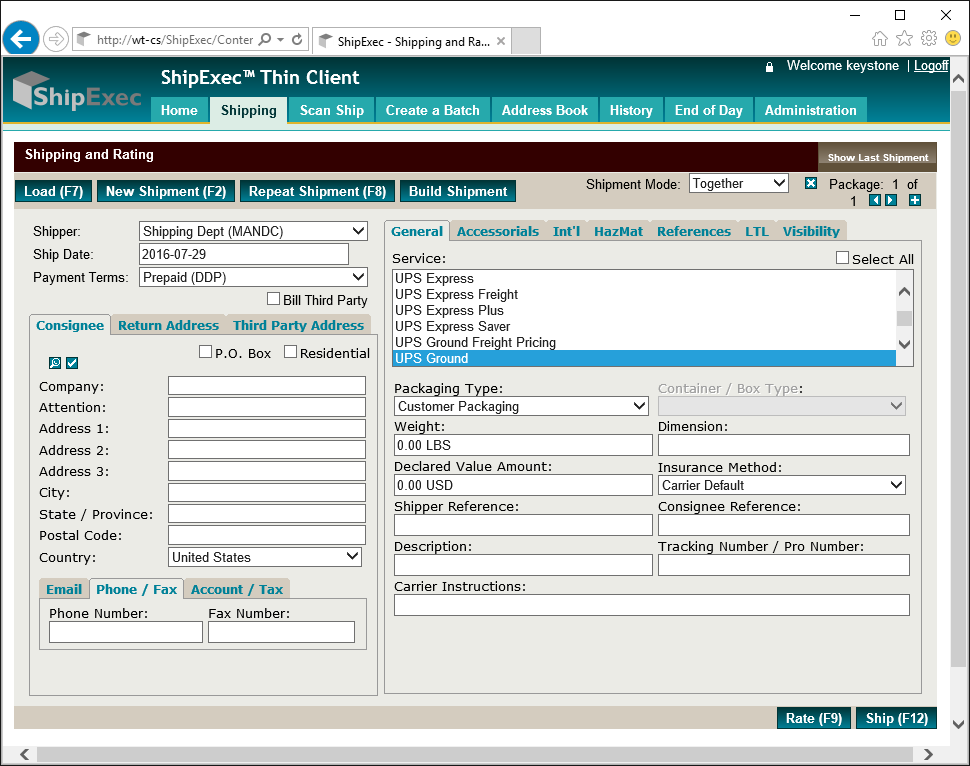
\includegraphics[width=\textwidth]{../img/image44}
\caption{ConnectShip Order Review and Ship}
\end{figure}

If an exception occurs during processing, the order is to be placed to the side, and the next order is to be shipped.

\pagebreak

\subsection{Receiving}

Receiving is used to update the warehouse with goods received from the vendor on a purchase order. Typically the vendor will send the product to the warehouse with a packing slip which includes an itemized list of the delivery contents. The vendor packing slip is then verified to the product to confirm that it is correct. The product would then be entered into \texttt{PORCV} for receiving. The receiving is a two step process which requires you to enter in the purchase order receipt \texttt{PORCV} and then post or update the inventory to the warehouse using \texttt{WAPOST}

\subsubsection{Inventory Receipts}

\index{ERP-One Commands!PORCV}

The command \texttt{PORCV} is used to access Inventory Receipts.

Enter in the purchase order number, then hit enter on the keyboard. You can also use F1 to look up the purchase order using the search tool.

You will be presented with a dialog box that allows you to select how you are receiving this order.

\begin{itemize}
	\item Item Selection
	\begin{itemize}
		\item Only Open Line Items \textemdash Only open lines on the PO will be listed
		\item All Line Items \textemdash All line times that have and have not been received on this PO will be listed
	\end{itemize}
	\item Default Quantity
	\begin{itemize}
		\item Zero \textemdash Quantity will default to zero
		\item Quantity Open \textemdash Quantity will default to expected amount remaining on PO
	\end{itemize}
\end{itemize}

After making the selection the purchase order will be listed on the screen. You will now need to enter the actual quantity received. If you selected Zero Default Quantity you will need to enter each line, if you chose Quantity Open you will need to verify the values shown.

The quantity still backordered after receipt will be shown in the entry field. If you wish to mark the order complete, simply change the backorder quantity to zero and the purchase order will be marked complete when hitting accept.

If the item is linked to a sales order, you will see, in red, the quantity linked from the receipt to the sales order.

If the item is only located, you will get a popup for assigning location.

\begin{enumerate}
	\item Type in how many you are assigning to that location
	\item If you are receiving to multiple locations, save the first location then click the next button at the top
	\item After you have assigned all quantities, click save then exit the popup	
\end{enumerate}

If the item is lot controlled and located, after entering the received quantity an additional screen will be shown for you to assign the location and lot number.

\begin{enumerate}
	\item Depending on the location type of the item, it may default to the receiving location. If you want to change the location, you can choose from the left side of the screen and click on the location
	\item If it is lot controlled, you will now assign a lot number unless the system is configured to auto assign a lot number
	\item Enter the quantity received against the lot and / or location
	\item Fill in other information as required
	\item Click save at the top of the screen
\end{enumerate}

If you are receiving into multiple locations, enter quantity to be received into the first location along with the lot information, then click save, and click next and repeat until finished.

\textbf{NOTE} You can use F1 in the location field to search for the location.

When you are finished receiving the order, click accept to begin the next receipt and apply the current one.

Bottom Buttons:

\begin{itemize}
	\item Add \textemdash Add additional items to the receipt if they were not on the original PO
	\item Delete \textemdash Delete the item from the receipt, this does not delete the item from the original PO
	\item Print Label \textemdash This will allow you to print a receiving label for what has been received
	\item Notes \textemdash This will allow you to enter item level notes
	\item Inquiry \textemdash Opens \texttt{WAINQ} for highlighted item
	\item Loc / Lot \textemdash If the item is located or lot controlled, this will reopen the Lot / Location information screen
	\item Add On's \textemdash This allows you to add additional costs to the purchase order
	\item Discrepancy \textemdash This will allow you to add a discrepancy to the receipt which is reportable
	\item Cancel \textemdash Cancel the receipt
\end{itemize}

To modify a receipt after it has been created in \texttt{PORCV} you will use \texttt{PORCVM}. This functions like \texttt{PORCV} but allows the modification of accepted receipts before posting.

\textbf{NOTE} If \texttt{XO} option porcv\_auto\_post has been set to 'yes', \texttt{WAPOST} will automatically open after accepting a receipt.

If the option to automatically post is active, you will be presented with the following options:

\begin{itemize}
	\item Run Allocation? \textemdash This will allocate the receipt to any open back orders
	\item Run Allocation from Whse? \textemdash This will also allocate stock found in the warehouse unrelated to this receipt
	\item Print Pick Tickets? \textemdash This allows you to print pick tickets if any back orders can be filled from recepit
	\item Print Post Report? \textemdash This allows you to print a report of what was received with location detail, lot information, etc. If this is checked, you will be prompted to print the post report
\end{itemize}

To print the picking slips, if any shipments were made possible through the new allocations, \texttt{OEPS} automatically opens. Refer to the section on printing picking slips.

\subsubsection{Receiving Reports}

The following reports are used to assist receiving:

\index{ERP-One Commands!PORPT}
\index{ERP-One Commands!RWS}
\index{ERP-One Commands!POREC}

\begin{itemize}
	\item \texttt{PORPT} \textemdash Open purchase order information
	\item \texttt{RWS} \textemdash Prints a receiving worksheet for open purchase orders
	\item \texttt{POREC} \textemdash Received purchase order information
\end{itemize}

\subsubsection{Warehouse Post}

\index{ERP-One Commands!WAPOST}

Items are not received into the warehouse until they have been posted. The \texttt{WAPOST} command allows you to post receipts into inventory.

\begin{itemize}
	\item Selections Tab \textemdash Set the options for the posting here
	\begin{itemize}
		\item Enable PO Receiving \textemdash This pulls all purchase orders that have been received so you can post them the the warehouse
		\item Enable Allocation \textemdash This will allocate the stock to backordered items on sales orders based on the allocation sort order you choose. If this is not checked then the orders will stay in a backorder status until someone commits them directly from \texttt{OE} or \texttt{OECHR}
	\end{itemize}
	\item Review \& Post \textemdash Create the list of receipts to be posted
	\begin{itemize}
		\item Under "Receiving Info" items to be received will be displayed, check items to be posted, or use "Select All" or "DeSel All" to manage the selection
		\item Under "Allocation Info" backorders that will be filled from this receipt will be displayed, check items to be allocated, or use "Select All" or "DeSel All" to manage the selection
		\item The "Inquiry" button located to the left will open \texttt{WAINQ} for the highlighted item
		\item The "History" button located on the bottom will allow you to review previous postings. \texttt{WARUH} may also be used to view warehouse post history.
		\item You may print a report here by clicking the "Print" button, or you can print the report later in \texttt{WARUH} after posting
		\item The "Cancel" button located on the bottom will cancel the transaction before posting occurs
	\end{itemize}
\end{itemize}

When you are ready to post the selected transactions, click "Post" located to the left of the screen.

\subsection{Dimensioning New Items (Cubiscan)}

\index{cubiscan}

When new items arrive in the building, an example of each should be directed to the person who will be responsible for dimensioning the item using the portable Cubiscan.

\subsubsection{Starting the Cubiscan}

\begin{enumerate}
	\item Ensure that the device is plugged in
	\item Ensure that the power inverter is turned on (display will be on)
	\item Turn on PC
	\item Turn on Cubiscan
	\item After the PC has started, open the QMI application
\end{enumerate}

\subsection{Scanning an Item}

\begin{enumerate}
	\item Ensure that the cubiscan is at zero.
	\begin{itemize}
		\item If fluctuating, check for vibrations or wind around the device
		\item If out of zero, clean glass and remove any obstructions, and press Zero on the Cubiscan display
	\end{itemize}
	\item Ensure that the gate is reset to the home position
	\item With the cursor in the item number field, scan the barcode of the item
	\item Place the item on the glass and then move the gate steadily to the other side and back
	\item On the application screen, ensure that the values have been recorded
	\item Press F4 to save data for the item
\end{enumerate}